\textbf{Date:} June 4th 2014\\\textbf{Duration:} 8-16\\\textbf{Group
members:} Henrik, Jakob, Jesper	

\subsection{Goals}

\begin{itemize}
\itemsep1pt\parskip0pt\parsep0pt
\item
  Get the robot to recognize cross sections
\item
  Get the vehicle to rotate solar panels
\item
  Get the vehicle to move around solar panels
\end{itemize}

\subsection{Results}

We keep having inconsistent turns, even using the power of mathematics
does not do the trick. We tried moving the front wheels further apart to
see if that would make the turns more accurate, but it did not help.
Instead, we replaced the front wheels with these smooth pads that allow
the vehicle to glide around with little friction. We decided to use
these because we suspect the omni-directional wheels we used to use
generate too much friction and make our turns inaccurate. The pads were
inspired by a kind group of engineers working on the same project.\\We
have also expanded the grabbing mechanism so that it is easier to catch a
solar panel, and now the whole panel manipulation mechanism is working
quite well.

\begin{figure}[hbt]
  \centering
  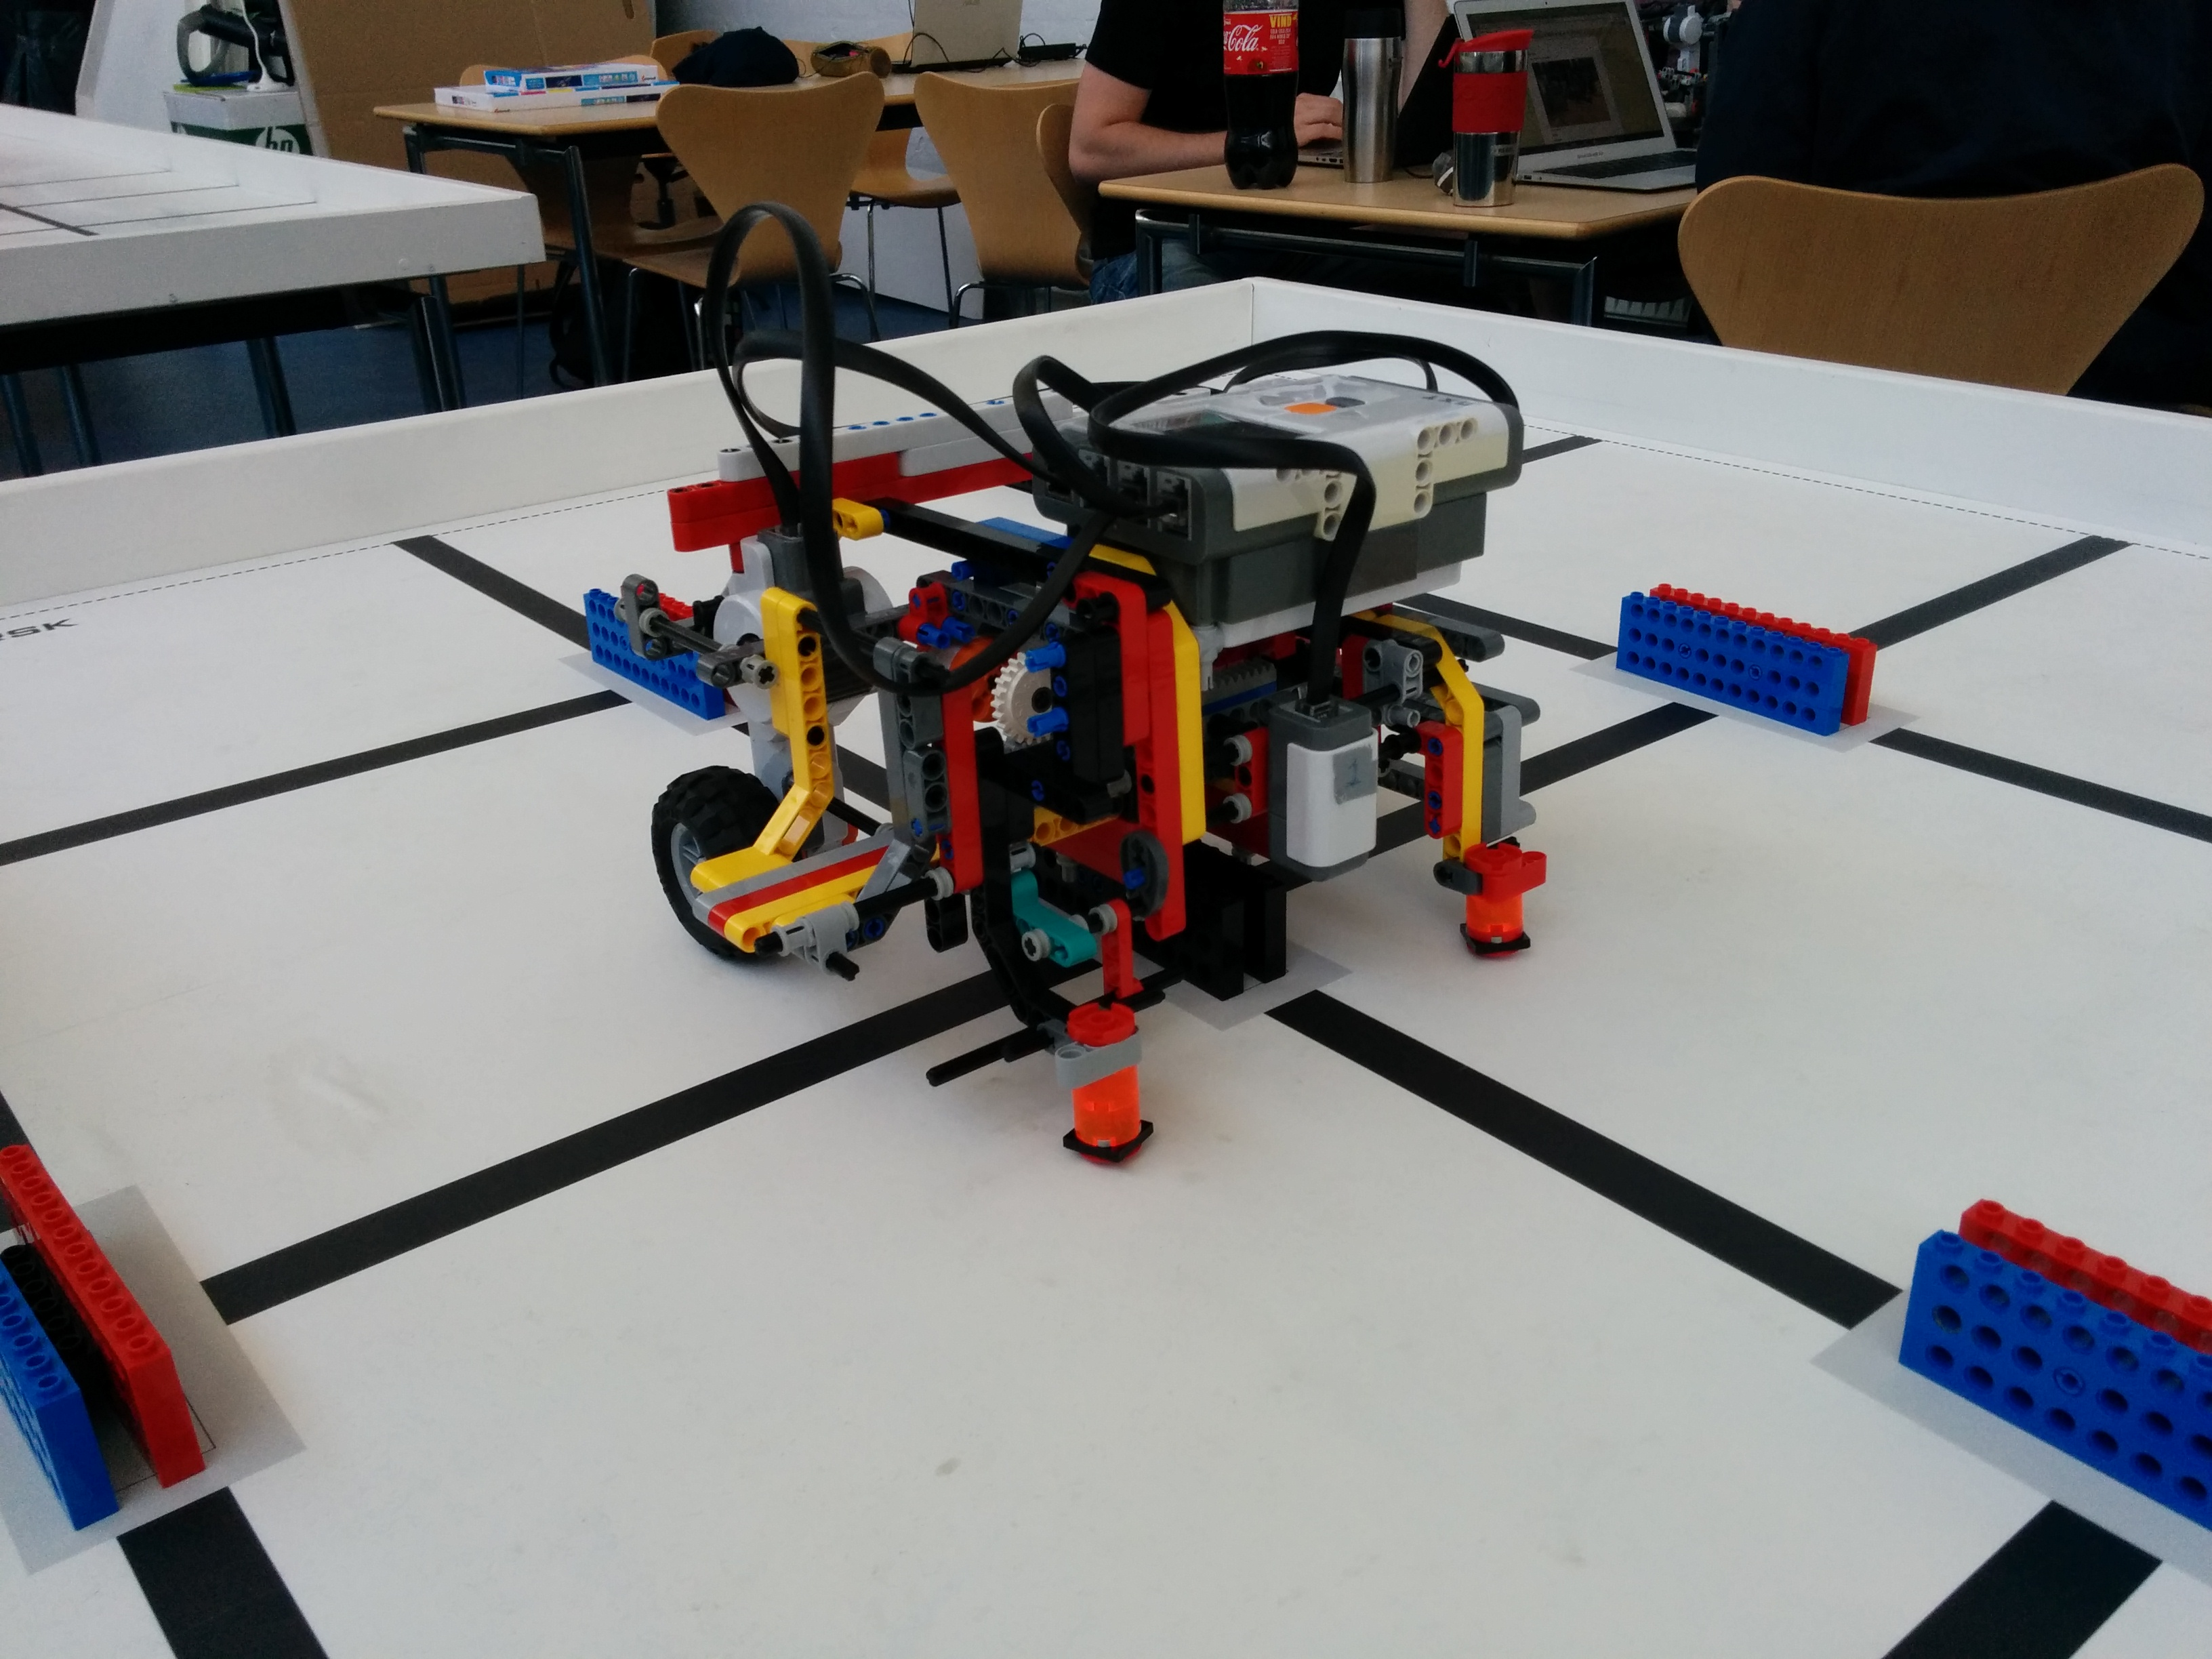
\includegraphics[scale=0.09]{../experiments/images/betterPrototype.jpg}
  \caption{Our prototype without front wheels.}
\end{figure}
\clearpage

We installed the color sensor today, to be used for registering what state a solar
panel is in. Initially it could not register colors, and saw everything
as black because of the distance to the panels. We will write our own
calibration for it.

We have been told that you can increase the accuracy of the light sensor
by placing a brick with holes in it in front of it. From an initial
test, we see that truly this is the case. However, positioning it
correctly using only LEGO bricks has proven to be incredibly difficult due to
the alignment of the holes. Therefore we have not included this in our
vehicle.

\subsection{Suggestions for easing the problem}

\begin{itemize}
\itemsep1pt\parskip0pt\parsep0pt
\item
  Make the track longer, giving our vehicle more room to turn. Our
  vehicle is a bit large, and when we rotate in order to turn a solar
  panel, we sometimes hit the adjacent panels.
\item
  We would like more time for the challenge. Two minutes is simply way too
  little time to both check the solar panels and rotate them, and to replace
  the defunct ones.
\item
  Have fixed lighting conditions, it is extremely difficult to
  calibrate the light sensor when the lighting keeps changing, differs
  from direction to direction, etc.
\end{itemize}

\subsection{Conclusion}

We still need to take care of the cross sections, but little by little
we have every part of a full run we need. The color sensor code has been
written, but needs testing.
